\documentclass[border=2pt]{standalone}
\usepackage{fontawesome5}\usepackage{xcolor}\usepackage{tikz}
\renewcommand{\familydefault}{\sfdefault}
\usetikzlibrary{positioning,calc,arrows.meta}
\definecolor{ink}{HTML}{1F2937}\definecolor{mute}{HTML}{6B7280}
\definecolor{gen}{HTML}{1B6CA8}\definecolor{expo}{HTML}{2E9E48}\definecolor{gxe}{HTML}{6A51A3}\definecolor{cov}{HTML}{9CA3AF}
\definecolor{resid}{HTML}{D8DCE1}\definecolor{prot}{HTML}{C0392B}
\begin{document}\begin{tikzpicture}[x=1cm,y=1cm,font=\sffamily,
  cic/.style={circle,minimum size=0.50cm,text=white,font=\fontsize{6.2}{6.2}\selectfont,inner sep=0pt},
  cl/.style={anchor=north,font=\fontsize{5.1}{5.5}\selectfont,align=center,inner sep=0.5pt}]
% green inflow stub from PXS (visual tie to the Sankey above)
\draw[-{Stealth[length=4.5pt]},expo,line width=1.2pt] (3.6,0.34) -- (3.6,-0.18);
\node[anchor=west,font=\fontsize{8.4}{8.8}\selectfont\bfseries,text=ink] at (0,0.02){HEAP variance partition};
\node[anchor=west,font=\fontsize{5.5}{6}\selectfont,text=mute] at (0,-0.40){PXS is one of four components of each plasma protein's variance};
% "one plasma protein's variance (100%)" removed 2026-08-31 (author): the
% line above already says the bar is one protein's variance.
% stacked variance bar
\def\by{-1.30}\def\bh{0.52}
\fill[cov]   (0.00,\by) rectangle ++(1.45,\bh);
\fill[gen]   (1.45,\by) rectangle ++(1.30,\bh);
\fill[expo]  (2.75,\by) rectangle ++(1.70,\bh);
\fill[gxe]   (4.45,\by) rectangle ++(0.90,\bh);
\fill[resid] (5.35,\by) rectangle ++(1.05,\bh);
\draw[white,line width=0.6pt] (1.45,\by)--++(0,\bh) (2.75,\by)--++(0,\bh) (4.45,\by)--++(0,\bh) (5.35,\by)--++(0,\bh);
\draw[expo,line width=1.0pt] (2.75,\by) rectangle ++(1.70,\bh);
\node[anchor=center,font=\fontsize{5}{5}\selectfont,text=mute] at (5.875,\by+0.26){$\varepsilon$};
\node[anchor=north,font=\fontsize{4.8}{5.2}\selectfont,text=mute,align=center] at (5.875,\by-0.05){noise /\\error};
% component icons + labels
\node[cic,fill=cov]  at (0.725,-1.92){\faSlidersH};\node[cl,text=cov]  at (0.725,-2.22){Covariates};
\node[cic,fill=gen]  at (2.100,-1.92){\faDna};     \node[cl,text=gen]  at (2.100,-2.22){Genetics\\\textcolor{mute}{PGS}};
\node[cic,fill=expo] at (3.600,-1.92){\faLeaf};    \node[cl,text=expo] at (3.600,-2.22){Exposures\\\textcolor{mute}{PXS}};
\node[cic,fill=gxe]  at (4.900,-1.92){\faProjectDiagram};\node[cl,text=gxe] at (4.900,-2.22){G$\times$E\\\textcolor{mute}{GIS}};
\end{tikzpicture}\end{document}
